\documentclass[a4paper,12pt]{article}
\usepackage[utf8]{inputenc}
\usepackage{graphicx}
\usepackage{array}
\usepackage{booktabs}
\usepackage{tabularx}
\usepackage{makecell}
\usepackage{float}
\usepackage{url}
\usepackage{listings}
\usepackage{xcolor}
\usepackage[czech]{babel}
\usepackage[unicode]{hyperref}
\newcommand{\centered}[1]{\begin{tabular}{l} #1 \end{tabular}}
\newcommand{\unit}[1]{\ensuremath{\, \mathrm{#1}}}
\addto\captionsczech{\renewcommand{\refname}{Seznam použité literatury}}
\addto\captionsczech{\renewcommand{\figurename}{\textbf{Obrázek}}}
\addto\captionsczech{\renewcommand{\tablename}{\textbf{Tabulka}}}
\renewcommand{\lstlistingname}{\textbf{Kód}}

\lstset{
    language=Python,
    basicstyle=\ttfamily\footnotesize,  % Zmenšené písmo
    keywordstyle=\color{blue},
    commentstyle=\color{gray},
    stringstyle=\color{red},
    numbers=left,
    numberstyle=\tiny\color{gray},
    stepnumber=1,
    breaklines=true,
    frame=single
}

\begin{document}
\vspace{\fill}
\begin{center}
    \renewcommand{\arraystretch}{1.75}
    \begin{tabularx}{\textwidth}{|X|X|X|}
        \hline
        \multicolumn{1}{|c|}{\rule{0pt}{2.25cm} 
\includegraphics[height=2cm]{img/ctu_logo.png}} & 
        \multicolumn{2}{c|}{\makecell{\textbf{KATEDRA FYZIKY}}} \\
        \hline
        \multicolumn{3}{|c|}{\Large \textbf{\centered{LABORATORNÍ CVIČENÍ Z FYZIKY}}} \\
        \hline
        \multicolumn{2}{|X}{\small{Jméno} \newline \textbf{Pavel Pernička}} & \multicolumn{1}{|X|}{\small{Datum měření} \newline \textbf{20.3.2025}} \\
        \hline
        {\small{Semestr} \newline \textbf{Letní 2025}} & {\small{Ročník} \newline \textbf{1.}} & {\small{Datum odevzdání} \newline \textbf{3.4.2025}} \\
        \hline
        {\small{Stud. skupina} \newline \textbf{6}} & {\small{Lab. skupina} \newline \textbf{1031}} & {\small{Klasifikace} \newline}\\
        \hline
        \multicolumn{3}{|c|}{\rule{0pt}{1cm}} \\
        \hline
        \multicolumn{1}{|X|}{\small{Číslo úlohy \newline \textbf{6}}} &
        \multicolumn{2}{|p{6cm}|}{\small{Název úlohy \newline \textbf{Měření permitivity dielektrik}}} \\

        \hline
    \end{tabularx}
\end{center}

\newpage

\section{Úkol měření}

\begin{itemize}
    \item Změřte relativní permitivitu jednoho, nebo dvou dielektrických vzorků.
    \item Pro každý vzorek (pokaždé do jednoho grafu) vyneste závislost náboje kondenzátoru na napětí v případě, kdy mezi deskami kondenzátoru je a není umístěn dielektrický vzorek.
\end{itemize}
\section{Seznam použitých přístrojů}
\begin{itemize}
    \item Zdroj vysokého napětí
    \item Měřicí zesilovač
    \item Ručičkový voltmetr
        \begin{itemize}
        \item Třída přesnosti: $2,5$
    \end{itemize}
    \item Dielektrické vzorky
        \begin{itemize}
        \item Červený plastový plát: $d_{č} = 10 mm$
        \item Průhledný plastový plát: $d_{p} = 8,6 mm$
    \end{itemize}
    \item Referenční kondenzátor
        \begin{itemize}
        \item Kapacita: $C_{REF} = 0,22 \mu F$
    \end{itemize}
\end{itemize}
\section{Měření}
\subsection{Postup}
\begin{enumerate}
    \item Zdrojem vysokého napětí nabijeme přes ochranný rezistor experimentální kondenzátor s~měřeným dielektrikem.
    \item Pomocí přepínače odpojíme experimentální kondenzátor od zdroje vysokého napětí a~přepojíme jej na referenční kondenzátor, která takto nabijeme.
    \item Pomocí ručičkového voltmetru změříme přes měřicí zesilovač napětí na referenčním kondenzátoru.
    \item Pomocí přepínače odpojíme referenční kondenzátor od experimentálního kondenzátoru, vybijeme referenční kondenzátor a celý proces opakujeme pro další napětí, s posunem o 500 V.
\end{enumerate}

\subsection{Tabulky naměřených hodnot}
Naměřené hodnoty napětí $U_X$ na paralelně spojeném referenčním kondenzátoru s experimentálním kondenzátorem při nabití experimentálního kondenzátoru zdrojem vysokého napětí s nastavením $U_z$ jsou znázorněny pro jednotlivé materiály dielektrika tabulkami níže. Náboj $Q$ kondenzátoru byl z naměřených hodnot vypočten pomocí vztahu:
$$
Q = C_{REF} \cdot \frac{U_Z \cdot U_X}{U_Z-U_X} = 0,22 \cdot 10^{-6} \cdot \frac{U_Z \cdot U_X}{U_Z-U_X} \unit{[C]}
$$

\begin{table}[H]
    \centering
    \renewcommand{\arraystretch}{1.5}
    \begin{tabular}{|c|c|c|c|c|}
        \hline
         & \multicolumn{2}{c|}{\textbf{Červené dielektrikum}} & \multicolumn{2}{c|}{\textbf{Vzduch}} \\
        \hline
        \rule{0pt}{1cm} \makecell{$\mathbf{U_z}$ [V]} & \makecell{$\mathbf{U_x}$ [V]} & \makecell{$\mathbf{Q}$ [C] \\ (vypočteno)} & \makecell{$\mathbf{U_x}$ [V]} & \makecell{$\mathbf{Q}$ [C] \\ (vypočteno)} \\ \hline
        500  & 0,56  & $1,23 \cdot 10^{-7}$  & 0,22 & $4,84 \cdot 10^{-8}$  \\ \hline
        1000  & 1,00  & $2,20 \cdot 10^{-7}$  & 0,38 & $8,36 \cdot 10^{-8}$  \\ \hline
        1500  & 1,45  & $3,19 \cdot 10^{-7}$  & 0,56 & $1,23 \cdot 10^{-7}$  \\ \hline
        2000  & 1,95  & $4,29 \cdot 10^{-7}$  & 0,74 & $1,62 \cdot 10^{-7}$  \\ \hline
        2500  & 2,6  & $5,72 \cdot 10^{-7}$  & 0,91 & $2,00 \cdot 10^{-7}$  \\ \hline
        3000  & 2,92  & $6,43 \cdot 10^{-7}$  & 1,15 & $2,53 \cdot 10^{-7}$  \\ \hline
        3500  & 3,50  & $7,70 \cdot 10^{-7}$  & 1,25 & $2,75 \cdot 10^{-7}$  \\ \hline
        4000  & 4,00  & $8,80 \cdot 10^{-7}$  & 1,40 & $3,08 \cdot 10^{-7}$  \\ \hline
        4500  & 4,40  & $9,68 \cdot 10^{-7}$  & 1,60 & $3,52 \cdot 10^{-7}$  \\ \hline
        5000 & 4,95  & $1,09 \cdot 10^{-6}$  & 1,75 & $3,85 \cdot 10^{-7}$  \\ \hline
    \end{tabular}
    \caption{Naměřené hodnoty pro červené plastové dielektrikum při šířce dielektrika $d_{č}=10mm$}
    \label{tab:rozmery_telesa}
\end{table}

\begin{table}[H]
    \centering
    \renewcommand{\arraystretch}{1.5}
    \begin{tabular}{|c|c|c|c|c|}
        \hline
         & \multicolumn{2}{c|}{\textbf{Průhledné dielektrikum}} & \multicolumn{2}{c|}{\textbf{Vzduch}} \\
        \hline
        \rule{0pt}{1cm} \makecell{$\mathbf{U_z}$ [V]} & \makecell{$\mathbf{U_x}$ [V]} & \makecell{$\mathbf{Q}$ [C] \\ (vypočteno)} & \makecell{$\mathbf{U_x}$ [V]} & \makecell{$\mathbf{Q}$ [C] \\ (vypočteno)} \\ \hline
        500  & 0,74  & $1,63 \cdot 10^{-7}$  & 0,24 & $5,28 \cdot 10^{-8}$  \\ \hline
        1000  & 1,45  & $3,19 \cdot 10^{-7}$  & 0,42 & $9,24 \cdot 10^{-8}$  \\ \hline
        1500  & 2,10  & $4,62 \cdot 10^{-7}$  & 0,60 & $1,32 \cdot 10^{-7}$  \\ \hline
        2000  & 2,85  & $6,27 \cdot 10^{-7}$  & 0,79 & $1,73 \cdot 10^{-7}$  \\ \hline
        2500  & 3,45  & $7,60 \cdot 10^{-7}$  & 0,98 & $2,15 \cdot 10^{-7}$  \\ \hline
        3000  & 4,10  & $9,03 \cdot 10^{-7}$  & 1,20 & $2,64 \cdot 10^{-7}$  \\ \hline
        3500  & 4,90  & $1,07 \cdot 10^{-6}$  & 1,40 & $3,08 \cdot 10^{-7}$  \\ \hline
        4000  & 5,60  & $1,23 \cdot 10^{-6}$  & 1,55 & $3,41 \cdot 10^{-7}$  \\ \hline
        4500  & 6,10  & $1,34 \cdot 10^{-6}$  & 1,70 & $3,74 \cdot 10^{-7}$  \\ \hline
        5000 & 7,10  & $1,56 \cdot 10^{-6}$  & 1,90 & $4,18 \cdot 10^{-7}$  \\ \hline
    \end{tabular}
    \caption{Naměřené hodnoty pro průhledné plastové dielektrikum při šířce dielektrika $d_{p}=8,6mm$}
    \label{tab:rozmery_telesa}
\end{table}

\section{Grafy}
\begin{figure}[H]
    \centering
    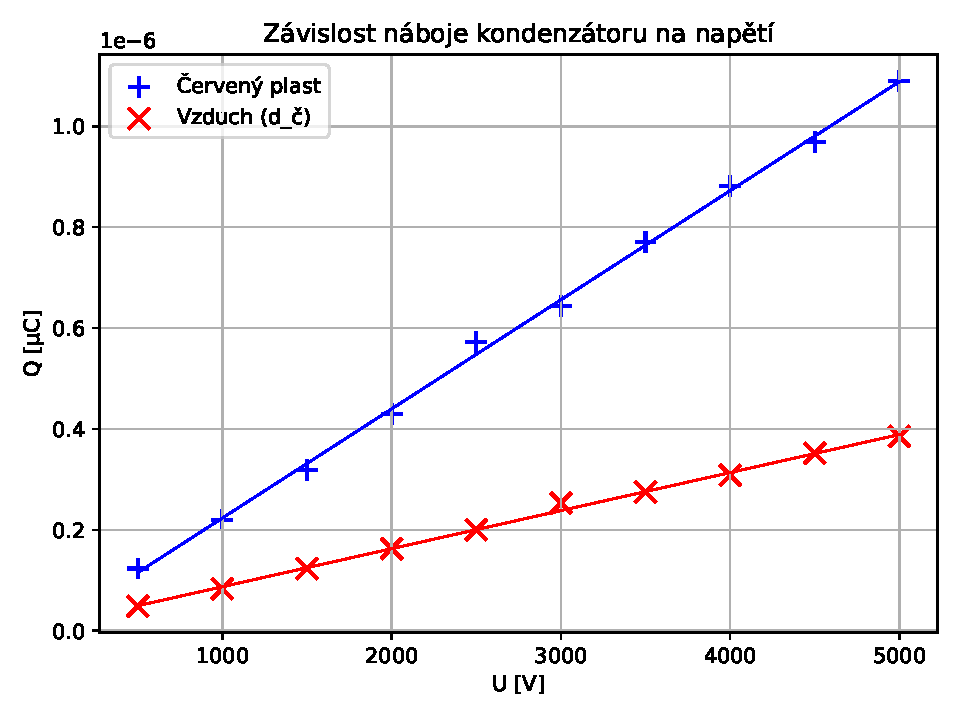
\includegraphics[width=0.95\textwidth]{img/cerveny_plast.pdf}
    \caption{Závislost náboje kondenzátoru na napětí pro červený plast a~vzduch při $d=d_{č}=10mm$}
    \label{fig:cerveny_plast}
\end{figure}

\begin{figure}[H]
    \centering
    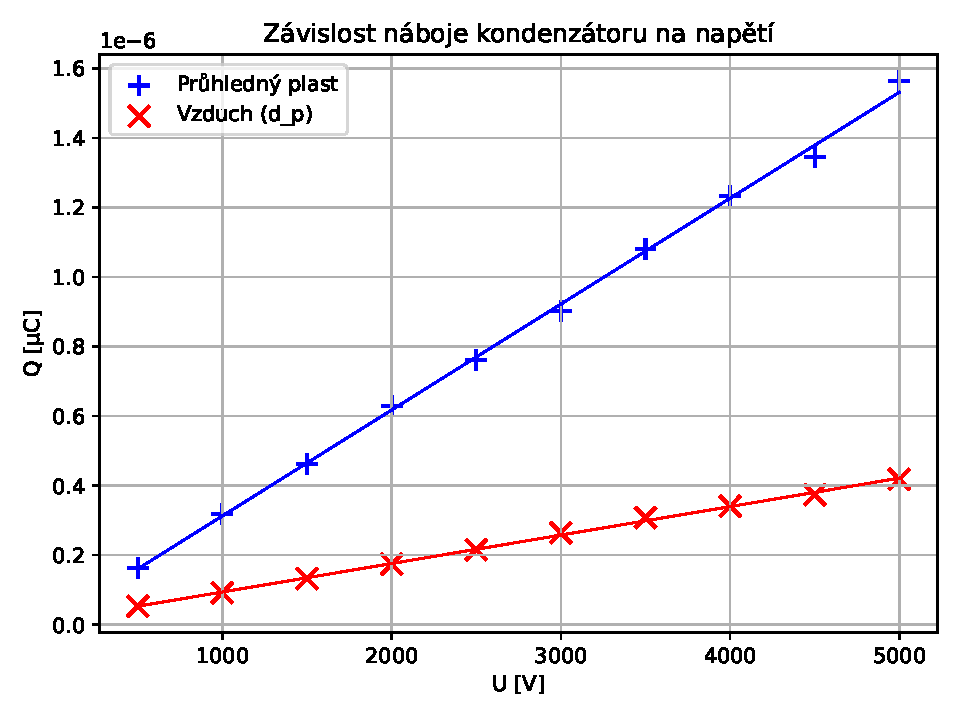
\includegraphics[width=0.95\textwidth]{img/pruhledny_plast.pdf}
    \caption{Závislost náboje kondenzátoru na napětí pro průhledný plast a~vzduch při $d=d_{p}=8,6mm$}
    \label{fig:pruhledny_plast}
\end{figure}


\section{Výpočty}
\subsection{Nejistota měření ručičkového voltmetru}
Vypočítáme ze vztahu pro nejistotu B analogových měřicích přístrojů z \cite{zpracdat}:
$$
u_B = \frac{2 \cdot R\cdot (TP/100)}{\sqrt{12}} = \frac{R\cdot (TP/100)}{\sqrt{3}} = \frac{10\cdot (2,5/100)}{\sqrt{3}} = 0,14
$$
Kde $R$ je rozsah přístroje a $TP$ je třída přesnosti přístroje.
\subsection{Kapacita kondenzátoru}
Kapacita kondenzátoru s různými dielektriky byla vypočítána pomocí Python skriptu metodou nejmenších čtverců při prokládání přímky skrze body v grafu. Jedná se o směrnice těchto proložených přímek. Nejistoty těchto směrnic byly určeny ze statistického rozptylu dat vzhledem k proložené přímce a zohledňují počet měření a rozložení hodnot napětí.

\begin{table}[H]
    \centering
    \renewcommand{\arraystretch}{1.5}
    \begin{tabular}{|c|c|}
        \hline
        \textbf{Dielektrikum} & \textbf{Vypočtená kapacita} \\ \hline
        Červený plast & $C_{č} = (216,29 \pm 2,87)[\unit{ pF}]$ \\ \hline
        Vzduch ($d = d_{č}$) & $C_{vč} = (75,43 \pm 1,32)[\unit{ pF}]$ \\ \hline
        Průhledný plast & $C_{p} = (304,66 \pm 4,27)[\unit{ pF}]$ \\ \hline
        Vzduch ($d = d_p$) & $C_{vp} = (81,89 \pm 1,10)[\unit{ pF}]$ \\  \hline
    \end{tabular}
    \caption{Přehled vypočtených kapacit pro různá dielektrika}
    \label{tab:out}
\end{table}

\subsection{Relativní permitivita kondenzátoru}
Relativní permitivitu vypočítáme jako poměr kapacity kondenzátoru s měřeným dielektrikem ($C$) a kapacity kondenzátoru pouze se vzduchem mezi elektrodami ($C_v$):
$$
\epsilon_r = \frac{C}{C_v} \quad \epsilon_{rč} = \frac{216,29}{75,43} = 2,86 \quad \epsilon_{rp} = \frac{304,66}{81,89} = 3,72
$$
\newpage
\subsection{Nejistota relativní permitivity kondenzátoru}
Nejistotu relativní permitivity určíme pomocí vztahu pro kombinovanou standardní najistotu, z něhož vyvodíme tento vzorec:
$$
    u(\varepsilon_r) =
    \sqrt{
        \left( \frac{1}{C_v} \right)^2 u(C)^2 +
        \left( \frac{C}{C_v^2} \right)^2 u(C_v)^2
    }
$$

Zde $u(C)$ a $u(C_v)$ jsou nejistoty kapacit určené při prokládání přímek, $C$~a~$C_v$ jsou ony kapacity.

\begin{itemize}
    \item Pro červený plast dosadíme:
$$
    u(\varepsilon_{rč}) &= \sqrt{
        \left( \frac{1}{75,43} \right)^2 \cdot 2,87^2 +
        \left( \frac{216,29}{75,43^2} \right)^2 \cdot 1,32^2
    } = \boxed{0,06}
$$

    \item Pro průhledný plast dosadíme:
$$
    u(\varepsilon_{rp}) &= \sqrt{
        \left( \frac{1}{81,89} \right)^2 \cdot 4,27^2 +
        \left( \frac{304,66}{81,89^2} \right)^2 \cdot 1,10^2
    } = \boxed{0,07}
$$
\end{itemize}
\section{Závěr}
V této laboratorní úloze jsme použili experimentální aparaturu složenou ze zdroje vysokého napětí, měřicího zesilovače, ručičkového voltmetru a referenčního kondenzátoru o známé kapacitě. Pomocí této soustavy jsme provedli sérii měření, při nichž jsme postupně určovali kapacitu deskového kondenzátoru s vloženými vzorky různých dielektrik, stejně jako v případě, kdy byl prostor mezi deskami vyplněn pouze vzduchem.

Na základě těchto měření jsme spočítali kapacitu experimentálního kondenzátoru v jednotlivých případech a z poměru těchto hodnot k měřením bez dielektrika jsme určili relativní permitivitu použitých dielektrik:

\begin{itemize}
    \item Červený plast: $\varepsilon_{rč} = (2,87 \pm 0,06)$
    \item Průhledný plast: $\varepsilon_{rp} = (3,72 \pm 0,07)$
\end{itemize}

Naměřené hodnoty relativních permitivit byly porovnány s tabulkovými hodnotami různých plastových materiálů. Hodnota $\varepsilon_r = (2,87 \pm 0,06)$ pro červený plast odpovídá přibližně hodnotám udávaným např. pro PTFE, PVC, nebo PP, které mají relativní permitivitu v rozmezí $2,5$ až $3,5$. Naměřená hodnota $\varepsilon_r = (3,72 \pm 0,07)$ se blíží hodnotám pro PEEK, nebo PEI (3,3 až 4,0). Na základě těchto údajů lze říci, že experimentální měření bylo dostatečně správné, protože nás dovedlo do odpovídající kategorie materiálů.

\begin{thebibliography}{}

    \bibitem{perm}
    Milan Červenka. \textit{Měření permitivity dielektrik}. Laboratorní úloha, 2013. Dostupné online: \url{https://planck.fel.cvut.cz/praktikum/downloads/navody/permitivita.pdf}.

    \bibitem{zpracdat}
    Milan Červenka. \textit{Zpracování fyzikálních měření}. Studijní text pro fyzikální praktikum, 2020. Dostupné online: \url{https://planck.fel.cvut.cz/praktikum/downloads/navody/zpracdat.pdf}.

\end{thebibliography}

\end{document}
